\chapter{Methods}\label{ch:methods}

\section{Overview}
Figure~\ref{fig:method} shows the steps of the evaluation. Trip records and survey answers were collected throughout the pilot, checked, analysed against the three goals, and reviewed with the scheme operator before this report was written.

\begin{figure}[htbp]
  \centering
  % Replace with your own figure: upload an image and change the file name below.
  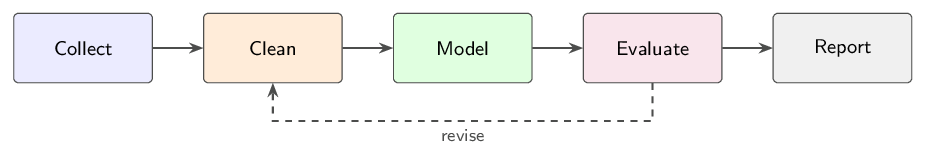
\includegraphics[width=0.9\textwidth]{figures/method.png}
  \caption{Steps of the evaluation.}
  \label{fig:method}
\end{figure}

\section{Trip Data}
Every docking station records the time at which a bicycle is released and returned. We received 73\,912 trip records from the operator. Records shorter than one minute or returned to the same station within three minutes were treated as failed releases and removed, which left 71\,460 trips.

\section{Measuring Use}
Use is reported as trips per bicycle per day,
\begin{equation}\label{eq:use}
  u = \frac{N}{B \times D},
\end{equation}
where $N$ is the number of trips, $B$ the number of bicycles in service and $D$ the number of days. Over the pilot, $B = 120$ and $D = 182$.

\section{Measuring Cost}
The net cost per trip is the operating cost less membership income, divided by the number of trips:
\begin{equation}\label{eq:cost}
  c = \frac{C_{\mathrm{op}} - I}{N}.
\end{equation}
Operating cost includes the operator's fee, maintenance and staff time. The purchase of bicycles and stations was funded by a separate grant and is not included.

\section{Survey}
All 1\,846 members were invited by email to complete a short survey in the final two weeks of the pilot; 412 did so, a response rate of 22\%. The key question asked how the respondent would have made their most recent trip if the scheme had not existed.
